\documentclass[LI,VKR]{HSEUniversity}
% Возможные опции: KR или VKR; LI

\title{Оценка применимости метода детектирования семантических изменений слов нейросетевой языковой моделью на основе генерируемых определений}
\author{Максим Дмитриевич Татаринов}
\supervisor{доцент факультета информатики, математики и компьютерных наук ВШЭ}{А. В.~Демидовский}
\reviewer{TBD}{П.П.~Петров}

\Year{2023}
\City{Нижний Новгород}

\Abstract{
 	Автоматическое обнаружение семантических изменений является областью исследований,
    вызывающей всё больший интерес из-за её важности для понимания эволюции языка и
    предоставления данных ключевым потенциальным пользователям,
    таким как лексикографы или историки языка.
    Ученые пытались зафиксировать семантические сдвиги, используя несколько методов,
    включая статические векторные представления слов, такие как Word2Vec (Фомин и др., 2019),
    более динамичные контекстуальные представления,
    такие как те, что создаются с помощью BERT или XML-R
    (Родина и др., 2020; Рачинский и др., 2021).
    Последние попытки использовали трансформеры с архитектурой кодировщика-декодировщика
    для генерации определений в качестве представлений смысла слов (Джулианелли и др., 2023).
    Несмотря на этот прогресс, остаётся нехватка исследований,
    сосредоточенных на русском языке с использованием этих передовых техник.
    Целью данного исследования является оценка применимости метода обнаружения
    семантических изменений в русском языке с использованием определений,
    сгенерированных языковой моделью.
    В данном исследовании предлагается использовать последние архитектуры
    трансформеров с кодировщиком-декодировщиком для моделирования определений для русского языка.
    Ожидаемым результатом исследования является достижение 80\% или более корреляции с аннотациями,
    созданными человеком, об обнаружении семантических изменений для русского языка.
}

\addbibresource{library.bib}

%%%%%%%%%%%%%%%%%%%%%%%%%%%%%%%%
%%% ТЕКСТ РАБОТЫ %%%%%%%%%%%%%%%
\begin{document}

% Обязательные элементы оформления: заголовочный слайд, аннотация, оглавление
\maketitle

\chapter*{Введение}


\textbf{Целью} настоящей работы является оценка применимости метода детектирования семантических
изменений слов нейросетевой языковой моделью на основе генерируемых определений.

Из поставленной цели были сформулированы следующие \textbf{задачи}:
\begin{enumerate}
    \item  Провести анализ существующей литературы и решений по задаче детектирования семантических
    изменений на основе генерируемых определений.
    \item  Собрать тезаурус русского языка в качестве материала для обучения модели, а также
    диахронический корпус текстов на основе НКРЯ.
    \item  Обучить языковую модель на данных тезауруса для того, чтобы генерировать определения.
    \item  Провести анализ метрик и качества обученной языковой модели и сравнить их с
    существующими решениями.
    \item  Создать алгоритм автоматического определения семантических сдвигов на основе их
    векторного представления.
    \item  Провести комплексный лингвистический анализ результатов работы компьютерной программы.
    \item  Разработать прототип системы, позволяющей проводить анализ семантических изменений
    сторонним исследователям, используя разработанный в настоящей работе алгоритм.
\end{enumerate}

\textbf{Объектом} исследования является метод детектирования семантических изменений слов.

\textbf{Предметом} исследования является применимость метода детектирования семантических изменений
слов с использованием нейросетевой языковой модели на основе генерируемых определений.

Для решения поставленных задач были использованы следующие \textbf{методы}:
\begin{enumerate}
    \item  Метод анализа и синтеза для создания теоретической базы для данного исследования на основе
литературы.
    \item  Компьютерный метод для написания алгоритмов программы и обучения модели.
    \item  Методы обработки естественного языка для предобработки текстов.
    \item  Методы машинного обучения для алгоритма автоматического определения семантических сдвигов на
основе их векторного представления.
    \item  Метод комплексного лингвистического анализа результатов работы алгоритма.
\end{enumerate}

На \textbf{актуальность} настоящей работы указывают следующие факторы.
Во-первых, активное изучение темы автоматического определения семантических изменений.
В последние годы в работах использовались различные методы, включая статические эмбеддинги,
контекстуальные эмбеддинги и заканчивая генерацией определений с помощью языковых моделей
в новейших исследованиях
~~\cite{kutuzov-etal-2018-diachronic,rodina2020elmo,DefinitionGenerationMainArticle}~.
При этом, абсолютное большинство исследований, посвященных моделированию определений,
проводятся с использованием материала английского языка~\cite{DefinitionModelingReviewAndDatasetAnalysis}.
Для русского языка вопрос анализа семантических изменений на основе автоматически
сгенерированных определений недостаточно изучен.
Во-вторых, неудовлетворительное качество традиционных методов для основных потенциальных
пользователей таких технологий, таких как лексикографы, историки языка и социологов.
Например, лексикографам недостаточно данных только о факте сдвига значения, им хотелось бы
получать описания старых и новых значений слов в пригодной для чтения форме, возможно,
даже с дополнительными пояснениями.
Данная проблема может решаться моделированием определений с использованием языковых
моделей, при использовании которых исследователи смогут получить более наглядные
результаты~\cite{DefinitionGenerationMainArticle}.

\textbf{Новизна} настоящей работы состоит в том, что для детектирования семантических изменений
значений слов применяется на материале русского языка и с использованием SOTA-моделей.

\textbf{Практическая значимость} данной работы заключается в том, что результаты настоящей работы
можно применять для определения степени семантического сдвига лексем, с наличием визуализаций и
определений для каждого выявленного значения, что может быть использовано в лексикологии,
где необходимы актуальные данные для построения новых словарей~\cite{DefinitionGenerationMainArticle}.
Кроме того, модель, позволяющая автоматически генерировать качественные словарные определения,
может быть полезна в таких задачах обработки естественного языка, как анализ тональности,
машинный перевод и разграничение семантической неоднозначности~\cite{DefinitionModelingReviewAndDatasetAnalysis}.

В качестве \textbf{материала исследования} используется диахронический корпус НКРЯ, охватывающий
три периода (1700—1916, 1918—1991 и 1992—2016 годы) и имеющий в совокупности 250 миллионов
словоупотреблений.
Данный корпус выбран, поскольку датасет слов для валидации с изменившимся и неизменившимся значением,
использующийся для оценки алгоритма, основан на данном корпусе~\cite{rushifteval}.
Корпус был получен по запросу к авторам НКРЯ.

\chapter{Теоретические аспекты автоматического выявления семантических изменений}

Традиционно для изучения изменений семантики слов использовались ручные методы детального
анализа текстов.
Хоть это и сохраняется в лингвистике, в последнее время появилось множество решений того,
как полуавтоматические и автоматические методы могут помочь расширить и
углубить такие исследования.
Одним из факторов, позволивший предлагать такие решения стала цифровизация документов
в различных областях и появление диахронических корпусов.

\section{Понятия и классификации}

В рамках изучения исторических изменений в лексике языка или языков, лингвисты оперируют
такими понятиями, как лексические изменения, семантические изменения,
грамматикализация и лексическая замена.

Лексические изменения в широком смысле охватывают все виды диахронических преобразований
в словарном составе языка, в то время как в более узком значении термин относится к
появлению новых форм в языке, таких как заимствованные слова и неологизмы,
а также к устаревшим словам.

Семантические изменения или семантический сдвиг являются особым случаем лексических изменений,
когда существующая форма (лексема) приобретает или теряет конкретное значение,
что приводит к увеличению или уменьшению полисемии.

Примером таких изменений может служить эволюция английских слов, когда ранее специализированное
слово для обозначения определенного вида собаки стало общим термином (dog),
в то время как более раннее общее слово для 'собаки' — современный аналог которого
hound — сейчас используется для обозначения специального вида собак.

Грамматикализация описывает особый вид семантических изменений, когда слова с
полным значением превращаются в служебные слова и, в конечном итоге,
в связанные грамматические морфемы.
Примером может служить развитие французского предлога chez из латинского существительного casa.
В случае и семантических изменений, и грамматикализации форма остается неизменной
— за исключением исторических фонетических сдвигов — в то время как ее содержание меняется.

В рамках настоящей работы мы будем заниматься исследованием семантических изменений,
не касаясь иных лексических изменений.

Одну из самых полных классификаций типов изменения семантики слова разработал немецкий
лингвист Г. Пауль (Пауль Г., 1960).
Он выделил следующие типы:

\begin{enumerate}
    \item Сужение значения, или специализация, при котором слово начинает употребляться
в более узких сферах общения за счет конкретизации своего значения.
Например, слово платье раньше означало «любую одежду, которую носят поверх белья»,
однако сейчас платье – «женская одежда особого покроя».
    \item Расширение значения, при котором значение слова становится более общим,
способным применяться во многих сферах общения.
Например, мошенник имел значение «вор-карманник», но теперь описывает
«любого нечестного на руку человека».
    \item Перенос значения, или метонимия, на основе смежности или близости ассоциативных связей.
Например, слово вздор изначально означало «то, что содрано при очистке дерева от коры;
стружки, хлам, отбросы», однако позже приобрело значение «бессмыслица, чепуха»
из-за ассоциативных связей.
    \item Метафора, заключающаяся в изменении значения на основе скрытого сравнения.
Например, глагол boil имел значение «пузыриться», позже по сходству характера действия получил
значение «кипятить».
    \item Возвышение значения,
при котором значение слова приобретает более позитивное значение в течение времени.
Например, слово chiffon обозначающее нежную деликатную воздушную ткань,
ранее имело значение «тряпка».
    \item Деградация значения,
когда значение слова приобретает более негативное значение в течение времени.
Например, слово gossip первоначально обозначало «крестного или крестную», а в современном языке
приобрело значение «сплетник, человек, рассказывающий скандальные истории другим людям».
    \item Гипербола, при которой значение слова нарочно преувеличивается.
    \item Литота, когда значение слова нарочно подвергается преуменьшению.
\end{enumerate}

\section{Обзор существующих методов}

\subsection{Cтатические эмбеддинги}

До 2020 года в работах чаще используют статические эмбеддинги.

Для русского языка в качестве примера можно привести проект Shiftry~\cite{shiftry},
в котором для анализа семантических сдвигов использовались модели Word2Vec,
выровненные методом Прокруста.
Эти модели были обучены на обширном корпусе русскоязычных новостных текстов,
охватывающем период с 2010 по 2020 годы, и позволили отследить диахронические изменения
в употреблении слов.
Для подсчета степени семантического сдвига использовалось косинусное расстояние между
векторами из различных временных срезов.

Статические эмбеддинги оставались наиболее актуальными вплоть до 2020,
где показывали лучшие результаты в SemEval-2020 Task 1~\cite{semeval2020task}.
Они эффективно моделируют значение слов в зависимости от обучающего корпуса
без опоры на объемные предобученные модели,
превосходя по этому качеству модели, основанные на совстречаемости слов.
Среди недостатков можно отметить необходимость большого объема слов в корпусах
для стабильности эмбеддингов;
необходимость выравнивания моделей, обученных на отдельных наборах данных,
соответствующим временным срезам, что может вносить шум;
кроме того, они моделируют среднее значение слова на основе его употребления в корпусе,
не позволяя различать разные значения слова.

\subsection{Контекстуализированные эмбеддинги}

Статические модели вложений слов присваивают каждому слову (лемме) один и тот же вектор
независимо от контекста, в то время как современные достижения в области обработки
естественного языка позволили разработать модели,
обеспечивающие получение контекстуализированных представлений высокого качества.
Данные модели отличаются тем, что на этапе вывода токенам присваиваются различные вложения
в зависимости от их контекста, что позволяет проводить более глубокий диахронический
анализ языковых изменений с использованием контекстуализированных векторных представлений слов.

Применение контекстуализированных векторных представлений задало новый стандарт для
высококачественных, чувствительных к контексту представлений в обработке естественного языка.
В статье, где исследователи использовали предварительно обученные модели BERT и ELMo,
настроенные на полном корпусе Русского национального корпуса, было обнаружено,
что эти модели показывают значительную корреляцию с человеческими оценками
при определении диахронического семантического изменения слов в русском языке~\cite{rodina2020elmo}.
Использовались алгоритмы, такие как косинусное сходство по прототипам слов и методы кластеризации,
для выявления семантических сдвигов.

Одни из последних работ по теме автоматического выявления семантических сдвигов для русского языка
были написаны в рамках соревнования RuShiftEval, прошедшего в 2021 году~\cite{rushifteval}.
В ходе него участники должны были рассмотреть три исторических периода русского языка и общества:
предсоветский (1700-1916), советский (1918-1990) и постсоветский (1992-2016).
Исследование базировалось на наборе данных RuShiftEval, который состоит из
111 русских существительных (99 в тестовом наборе и 12 в наборе для разработки),
вручную аннотированных по степени изменения их значения в трех парах временных периодов.

Аннотаторам предлагалось оценить семантическую связь значений целевого слова в двух предложениях
из разных временных периодов.
Оценки (от 1 до 4) отражали степень семантического родства между значениями слова, где
1 обозначало отсутствие связи между значениями, а 4 – их совпадение.
Затем индивидуальные оценки усреднялись, формируя общую меру семантической родственности между
употреблениями слова в разные временные периоды.
Такая задача как правило называется Word-in-Context или WiC.

Для каждого из 99 целевых русских слов участники должны
были представить три значения, соответствующих семантическому изменению в упомянутых парах
временных периодов.
Эти значения использовались для построения трех ранжирований:
RuSemShift1, RuSemShift2 и RuSemShift3.
В качестве метрики оценки использовалась ранговая корреляция Спирмена между ранжированием слов,
сгенерированным системой, и золотым ранжированием, полученным в ручной аннотации.

Победители вышеупомянутого соревнования (команда GlossReader) указывают,
что проблемой в существующих решениях являлось то,
что эмбеддинги несут в основном информацию о форме слова, а не значении~\cite{GlossReader}.
Чтобы решить это, они дообучали модель XLM-R на задаче генерации эмбеддингов, максимально близким
к таким, какие получены на соответстующим использованиям слов словарным определениям
~\cite{XLM-R}.

При дообучении их система включает в себя два отдельных энкодера на основе XLM-R:
Энкодер контектов для кодирования предложения с целевым словом и
энкодер глоссов для кодирования определения слова.
Система оценивает возможные значения смысла слова путём сравнения векторных представлений слова
и его определений.
При этом для обучения использовались данные только по английскому языку,
но модель также показала хорошие результаты для русского языка.

Далее, исследователи получали эмбеддинги контекстов слов с помощью
дообученного энкодера контекстов, высчитывали расстояние с помощью различных метрик расстояния,
самым эффективным из которых были евклидово расстояние с нормализацией, после чего
логистическая регрессия приводила значения к формату в датасете.

Авторы статьи предоставляют доступ к части исходного кода их исследования~\cite{GlossReaderGitHub}.

Так, были опубликованы следующие компоненты:
\begin{enumerate}
    \item Код, предназначенный для генерации прогнозов на основе заранее вычисленных эмбеддингов,
полученных с использованием модели.
    \item Код для оценки результатов.
\end{enumerate}

В то же время, авторы исследования не представили в открытый доступ следующие части:
\begin{enumerate}
    \item Код для предварительного обучения модели.
    \item Код, позволяющий осуществлять инференцию для получения контекстуализированных
    эмбеддингов, сформированных на основе предварительно обученной модели.
\end{enumerate}

В соответствии с инструкциями, данными авторами, мы запустили доступный код,
в следствие чего были полуены высокие результаты, совпадающие с тем, что сообщают
авторы в своей работе:

\begin{table}[htbp]
\centering
\caption{Коэффициэнты корреляции}
\begin{tabular}{lc}
\hline
Пары периодов                  & Коэффициент корреляции \\
\hline
Среднее            & 0.8021                  \\
pre-Soviet:Soviet           & 0.7808                  \\
Soviet:post-Soviet          & 0.8032                  \\
pre-Soviet:post-Soviet      & 0.8223                  \\
\hline
\end{tabular}
\end{table}

Среди недостатков работы можно отметить неспособность модели корректно выявлять
значения тех слов, которые отличаются от ближайших аналогов в английском, например,
\("\)пионер\("\), связанный с коммунистической идеологией и не соответствующий в полной мере
слову \("\)scout\("\).

Кроме того, команда DeepMistake представила решение, занявшее в соревнование второе место
~\cite{DeepMistake}.
Однако, они смогли доработать его и повысить результаты до первого уже после окончания
соревнования.

Исследователи обучали модель XLM-R на обширном многоязычном датасете Word-in-Context,
а затем дооубчали ее на наборе данных RuSemShift для настоящей задачи,
приводит к наилучшим результатам.
В отношении архитектуры авторы утверждают, что применение линейного слоя на верхнем уровне,
основанного на объединении L1-метрики и скалярного произведения между контекстуализированными
эмбеддингами XLM-R, показывает лучшую производительность по сравнению с
более традиционными подходами, такими как конкатенация эмбеддингов и
использование нелинейных классификаторов.

Исследователи выложили исходный код полностью и предлагают возможность воспроизвести их
результат~\cite{DeepMistakeGitHub}.
Значени метрик, сообщенные исследователями, воспроизводятся.

\begin{table}[htbp]
\centering
\caption{Коэффициэнты корреляции с использованием IsoReg}
\begin{tabular}{lc}
\hline
Пары периодов                  & Коэффициент корреляции \\
\hline
Среднее            & 0.8494                  \\
pre-Soviet:Soviet           & 0.8563                  \\
Soviet:post-Soviet          & 0.841                  \\
pre-Soviet:post-Soviet      & 0.8511                  \\
\hline
\end{tabular}
\end{table}

Среди недостатков статьи можно выделить то, что авторы не предоставляют возможность визуализации
или интерпретации результатов, кроме непосредственно получившегося значения метрики.

Тем не менее, применимость таких методов была подвергнута сомнению в работе
Giulianelli et al.~\cite{DefinitionGenerationMainArticle},
где ставится под сомнение широкая практичность ранее упомянутых подходов.
Они утверждают, что такие методы практически неинтерпретируемы,
поскольку они не дают описаний значений слов,
а лишь бинарные результаты наличия или отсутствия семантического изменения.
Исследование, которое в наибольшей степени занимается этой проблемой, - это GlossReader,
где исследователи предлагают способ визуализации и интерпретации результатов.
Однако у этого метода есть свои недостатки, обсуждаемые выше.
Учитывая эти факты, новый подход, включающий моделирование определений,
вызывает интерес для задачи обнаружения семантических изменений.

Начало интереса к моделированию определений как теме исследования
в области обработки естественного языка можно отнести
к работе Noraset et al.~\cite{noraset2016definition}.
Они были среди первых, кто исследовал потенциал использования векторных представлений слов
для автоматической генерации определений.
Изначально была поставлена упрощенная задача с моносемантическими словами,
которые, как правило, имеют одно значение и, следовательно, одно определение.
Однако оставалась нерешенной проблема многозначных слов.
Gadetsky et al. выделили важное условие для моделирования определений:
необходимость контекста для точного захвата нюансов языка~\cite{gadetsky-etal-2018-conditional}.
В своем исследовании они включили примеры предложений для предоставления контекста модели,
что оказалось решающим шагом в возможности модели справляться с полисемией и улучшении
ее производительности.

Несмотря на достижения, сделанные вышеупомянутыми исследователями,
область моделирования определений все еще сталкивалась с значительными проблемами.
Huang et al. выявили наличие таких проблем,
как проблема слов вне словаря, когда модели сталкиваются с трудностями в работе со словами,
не встречавшимися во время обучения, а также проблемы избыточной и недостаточной
специфичности в определениях~\cite{huang-etal-2021-definition}.
Исследователи сообщают: \("\)Избыточно специфичные определения представляют узкие значения слов,
в то время как недостаточно специфичные определения представляют общие и
нечувствительные к контексту значения.\("\)
Huang et al. решили эти проблемы,
используя предварительно обученную модель энкодера-декодера,
а именно Text-to-Text Transfer Transformer (T5),
и ввели механизм ранжирования, предназначенный для тонкой настройки специфичности
генерируемых определений.
Метод был протестирован на стандартных наборах данных для оценки и показал значительное
улучшение по сравнению с предыдущими методами.

Самой актуальной работой по теме использования сгенерированных большими языковыми моделями
определений для автоматического выявления семантических изменений является статья
Giulianelli et al.~\cite{DefinitionGenerationMainArticle}.

Авторы определяют задачу генерации определений следующим образом: для заданного слова w и примера
использования s (предложения, содержащего w) необходимо сгенерировать определение d на
естественном языке, которое будет грамматически корректным и точно передавать значение слова
w в контексте его использования.
Для генерации определений они используют модель Flan-T5, версию трансформера T5,
дополнительно обученную на 1,8 тысячах задач по обработке естественного языка.
Ниже вы можете видеть пример работы модели.

\begin{table}[htbp]
\centering
\caption{Пример определения, сгенерированного моделью Flan-T5 XL}
\begin{tabular}{|l|p{10cm}|}
\hline
\textbf{Пример использования} & ‘Примерно половина солдат в наших стрелковых взводах были призывниками, которых мы обучали около шести недель.’ \\
\hline
\textbf{Целевое слово} & призывник \\
\hline
\textbf{Сгенерированное определение} & ‘ЧЕЛОВЕК, КОТОРЫЙ ПРИЗВАН В ВООРУЖЕННЫЕ СИЛЫ’ \\
\hline
\end{tabular}
\end{table}

Первым шагом исследователи выбирают, используя метрики BLEU, NIST, BERTScore, наиболее
подходящий под задачу промпт из нескольких вариантов, например
\("\)what is the definition of <trg>?\("\) или \("\)define the word <trg>\("\).

Для дообучения модели авторы используют три датасета, каждый из которых содержит определения
слов, сопровождаемые примерами употребления: WordNet, данные Оксфордского словаря и CoDWoE,
основанный на определениях и примерах, извлеченных из Викисловаря.

Для оценки качества модели исследователи используют метрики SacreBLEU, ROUGE-L и BERT-F1.

Для демонстрации работы со сгенерированными определениями авторы
работы используют датасет, в котором слова представлены в графах диахронного использования
слов (Diachronic Word Usage Graphs, DWUG), взвешенных, ненаправленных графах,
узлами которых служат примеры использования слов, а веса рёбер отражают семантическую
близость пар употреблений.
DWUG созданы на основе многоэтапного процесса человеческой аннотации, в ходе которого аннотаторы
оценивали семантическую связность пар употреблений слов по 4-балльной шкале.

Прежде всего, авторы исследования проводят анализ корреляции между близостью пар слов в DWUG
и контекстуальными эмбеддингами токенов, эмбеддингами предложений примеров использования, а также
сгенерированными определениями.
Результаты показали, что сгенерированные определения обладают более высокой степенью
корреляции с данными из DWUG, чем традиционно полученные эмбеддинги.

Далее исследователи анализируют пространство эмбеддингов определений слов,
чтобы выяснить, как они могут помочь в различении разных значений слов.
Они обнаружили, что эмбеддинги определений образуют более плотные и четко определенные
кластеры по сравнению с эмбеддингами токенов и примеров предложений, что делает их
подходящими для представления значений слов.

Далее авторы присваивали кластерам, полученным на основе данных из DWUG,
соответствующие им определения.
Для обобщения определений в одном кластере авторы использовали самое прототипическое из них.
Они представляли все определения с помощью их эмбеддингов предложений и выбирали в качестве
прототипичного определение, эмбеддинг которого наиболее похож на среднее значение всех
эмбеддингов в кластере.

Авторы приходят к выводу, что сгенерированные определения слов могут играть роль
семантического представления слов, аналогичному традиционным эмбеддингам.
Они находят большие языковые модели достаточно развитыми для генерации определений
простым промптом.
При этом полученные таким образом определения превосходят по качеству
традиционные эмбеддинги и являются более наглядными.

\chapter{Имплементация автоматического выявления семантических изменений}

\section{Обучение языковой модели на данных тезауруса}

В качестве модели была выбрана FRED-T5-1.7B, являющаяся одной из новейших языковых моделей,
выпущенных SberDevices и обученных с нуля на материале русского языка~\cite{FRED-T5}.
Для выбора модели мы использовали бенчмарк для оценки продвинутого понимания русского языка
\("\)RussianSuperGLUE\("\)~\cite{RussianSuperGLUE}.В бенчмарке присутствуют шесть групп задач, охватывая
общую диагностику языковых моделей и различные лингвистические задачи: понимание здравого смысла, логическое
следование в естественном языке, рассуждения, машинное чтение и знания о мире.
FRED-T5-1.7B занимает самое высокое место в лидерборде данного бенчмарка, со значением 0.762,
уступая лишь результатам выполнения данных заданий людьми со значением 0.811,
что свидетельствует о ее способности к выдающемуся языковому пониманию и анализу.
Таким образом, FRED-T5-1.7B представляется наиболее подходящей языковой моделью
для задачи генерации определений.

Одной из ключевых особенностей модели FRED-T5-1.7B является наличие денойзеров.
Денойзеры — это специальные механизмы, задача которых состоит в очистке текста от шума,
то есть в восстановлении удаляемых или искажаемых частей текста.
В модели используется семь различных денойзеров, каждый из которых выполняет
уникальную функцию в процессе обучения.
Основные задачи денойзеров включают в себя восстановление
удаленных участков текста (спанов), а также продолжение текстовых последовательностей.

В настоящей работе при работе с моделью используется денойзер,
помеченный спецтокеном \("\)<LM>\("\),
который задействован в задаче продолжения последовательности текста.

Действия, описанные далее, подкрепляются кодом, выложенным в открытый доступ, на сайте GitHub
и могут быть воспроизведены. (TODO: ВСТАВИТЬ ССЫЛКУ)

В качестве материала, используемого для обучения модели, выступила русская версия Викисловаря.
Материал получен с помощью написанного скрипта на языке Python, позволяющего
извлечь данные из выгрузки Викисловаря в формат JSONL, где в каждом вхождении присутствовали
идентификатор статьи, лексема, про которую написана данная статья, а также определения
с примерами использования.

\begin{longtable}{|m{3cm}|m{10cm}|}
\caption{Информация о лексеме из Викисловаря} \\
\hline
\textbf{Лексема} & \textbf{Определения и примеры использования} \\
\hline
\endfirsthead
\multicolumn{2}{c}%
{\tablename\ \thetable\ -- \textit{Продолжение с предыдущей страницы}} \\
\hline
\textbf{Лексема} & \textbf{Определения и примеры использования} \\
\hline
\endhead
\hline \multicolumn{2}{r}{\textit{Продолжение на следующей странице}} \\
\endfoot
\hline
\endlastfoot
прозябнуть & \textbf{сильно озябнуть, промёрзнуть:} Я и без того прозяб,
инстинкт тянет меня согреться, а какой-то нелепый долг повелевает лезть в холодную воду.
Усталость возьмет свое, тогда можно жестоко прозябнуть и опасно заболеть.
\newline \textbf{прорасти:} Сперва надо его в землю посадить, потом ожидать,
покуда в нем произойдет процесс разложения, потом оно даст росток, который прозябнет,
в трубку пойдет, восколосится и т. д. \\
\end{longtable}

Полученный материал был очищен от вхождений, не имеющих при себе примеров использования,
информативных определений или определений вовсе, а также имеющие такие определения,
которые представляют грамматическое значение вместо лексического.
На выходе было получено 185595 вхождений.

Примеры и слова были отформатированы под формат запроса модели.
В начале после слова \("\)Контекст\("\) шел пример использования слова, после чего шла фраза
\("\)Определение слова\("\), в которую включалось само слово.
Таким образом, на вход модель
принимает лексему и контекст, в которой она употреблялась, а на выход ожидается сгенерированное
определение.

\begin{table}[h]
\centering
\caption{Пример отформатированного запроса модели}
\begin{tabular}{|m{2.5cm}|m{9.5cm}|}
\hline
\textbf{Поле}       & \textbf{Значение}                                                                                          \\
\hline
input\_text  & <LM>Контекст: \("\)Усталость возьмет свое, тогда можно жестоко прозябнуть и опасно заболеть.\("\) Определение слова \("\)прозябнуть\("\): \\
\hline
target\_text & Сильно озябнуть, промёрзнуть.                                                                              \\
\hline
\end{tabular}
\end{table}

FRED-T5-1.7B была дообучена на полученном из Викисловаря материале в течение трёх эпох
с линейным шагом обучения 0.001, размером батча 16 и оптимизатором Adafactor.
Для ускорения обучения и экономии видеопамяти использовалась технология LoRa со
следующими параметрами: r – 16, alpha – 64, dropout – 0.1.
Более подробный обзор гиперпараметров модели доступен в приложении TODO: Написать приложение.

Для оценки качества обучения модели используются метрики BLEU и ROUGE-L,
которые оценивают формальную схожесть текста: BLEU оценивает точность совпадений n-грамм
в сгенерированном тексте по сравнению с эталонным текстом~\cite{BLUE}, а ROUGE-L измеряет схожесть между
сгенерированным текстом и эталонным текстом на основе наибольшей общей последовательности слов~\cite{ROUGE}.
Также использовалась метрика BERT-F1, учитывающая семантику сравниваемых текстов благодаря
использованию контекстуальных эмбеддингов при подсчете значения метрики~\cite{BERTScore}.
Использование нескольких метрик позволяет получить более полную картину качества модели,
поскольку каждая из них оценивает разные аспекты сгенерированного текста.
Как традиционные BLEU и ROUGE-L, так и более современный BERT-F1 активно используются в
задачах обработки естественного языка, в том числе в задачах генерации текста.
В данной работе использовались версии этих инструментов, взятые из библиотеки evaluate~\cite{Evaluate}.
Так, в обзорной статье по моделированию определений утверждается, что на момент выпуска статьи BLUE
использовался в 9 научных публикациях, ROUGE-L и BERTScore – в 3~\cite{DefinitionModelingReviewAndDatasetAnalysis}.
Кроме того, данные метрики используются и в более новых работах.
Так, в настоящей статье результаты данных метрик будут сравниваться с таковыми из статьи
Giulianelli M. et al., где сообщаются результаты трёх вышеперечисленных метрик при обучении модели
Т5 для задаче генерации определений на английском языке~\cite{DefinitionGenerationMainArticle}.

\begin{table}[htbp]
\centering
\caption{Результаты дообучения FRED-T5-1.7B на датасете Викисловаря}
\begin{tabular}{lc}
\hline
Метрика                  & Значение \\
\hline
BLEU            & 8.3162                  \\
ROUGE-L           & 37.45                  \\
BERT-F1          & 78.06                  \\
\hline
\end{tabular}
\end{table}

\section{Тестирование модели на материале соревнования Rushifteval}

С помощью модели были получены определения для тестовой части датасета соревнования Rushifteval.

Для векторизации сгенерированных определений использовалась rubert-tiny2,
векторы были нормализированы, после чего расстояние между
векторным представлением определений считалось с помощью косинусного расстояния.
Результат приводился в формат значений датасета с помощью линейной регрессии,
тренированной на датасете Rusemeval.

\begin{table}[htbp]
\centering
\caption{Коэффициэнты корреляции с использованием IsoReg}
\begin{tabular}{lc}
\hline
Пары периодов                  & Коэффициент корреляции \\
\hline
Среднее            & 0.6412                  \\
pre-Soviet:Soviet           & 0.6128                  \\
Soviet:post-Soviet          & 0.6703                  \\
pre-Soviet:post-Soviet      & 0.6403                  \\
\hline
\end{tabular}
\end{table}

Настоящее решение лучше по качеству большинства аналогов из соревнования Rushifteval,
хоть и уступает некоторым, использующим модели XLM-R.

\section{Визуализация результатов работы модели}

Для создания визуализаций семантических изменений слов используются используются библиотеки
Matplotlib и Scikit-learn.
Полученные с помощью модели определения векторизуются по аналогии с выше описанными главами.
Так как для слов, где значение в приведенном контексте одинаковое,
модель склонна генерировать семантичсеки близкие, однако не идентичные дословно определения,
для группировки таких схожих определений применяется алгоритм кластеризации DBSCAN из
библиотеки Scikit-learn на основе векторных представлений.
После этого, для каждого полученного кластера выбирается прототипическое определение,
векторное представление которого наиболее близко к центру кластера.
Кластеры, содержащие менее четырех примеров за все эпохи не являются достаточно информативными
и отбрасываются как выбросы.
Matplotlib применяется для создания столбиковых диаграмм,
отражающих частоту употреблений различных значений слова во времени,
и для обеспечения наглядности с помощью цветовой градации и легенд,
содержащих прототипические определения каждого из значений.

Как видно в примере на иллюстрации 2.1, визуализация слов из набора данных Rusemshift
позволяет наглядно выявлять семантические различия в словах в разных эпохи.

\begin{FIGURE}[h]{Изменение значений слова "Спутник" \label{fig:example-figure-2}}
	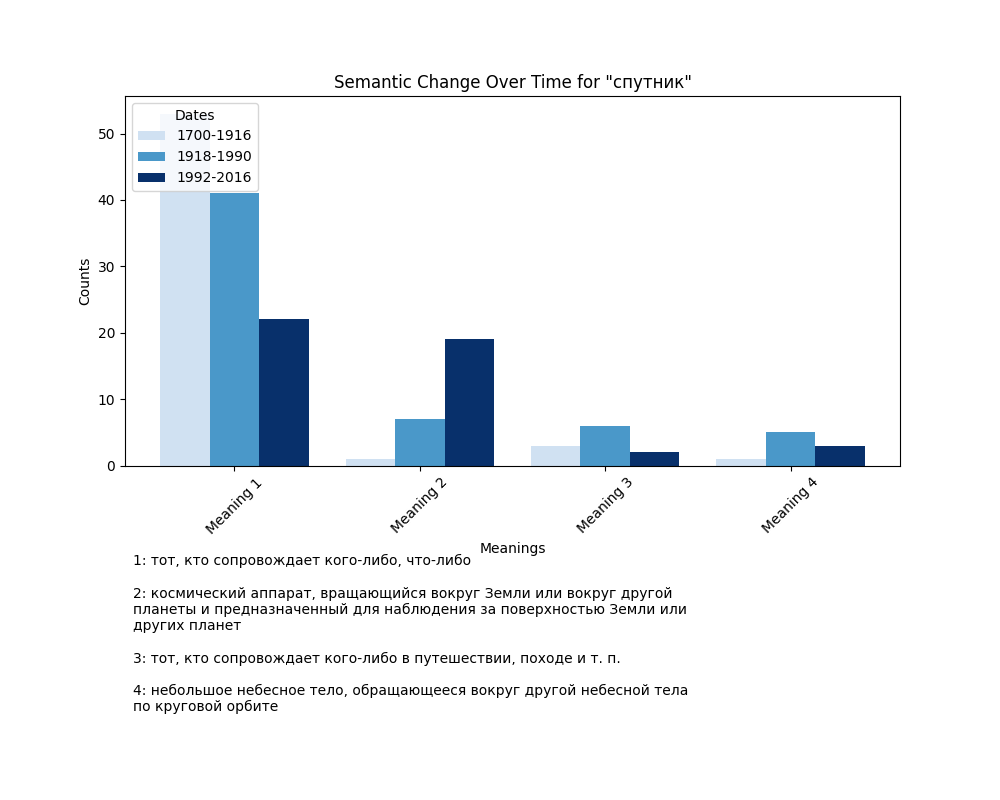
\includegraphics[width=1.0\textwidth]{img/Figure_Sputnik_2}
\end{FIGURE}

\chapter{Анализ результатов работы модели}

Для дальнейшего анализа результатов алгоритма использовались 20 слов с изменившемся
значением из книги «Два века в двадцати словах» [Данова et al, 2018].
Использования данных слов брались из диахронического корпуса НКРЯ.

\chapter*{Заключение}

Таким образом, в результате исследования моделирование определений может быть
успешно применено для задачи детектирования семантических изменений.
Несмотря на то, что представленное решение не является лидирующим по качеству,
оно имеет высокую степень интерпретируемости и предлагает один
из наиболее наглядных методов визуализации.
Результаты настоящей работы можно применять для определения степени семантического сдвига лексем,
с наличием визуализации и определений для каждого выявленного значения,
что может быть использовано в лексикологии,
где необходимы актуальные данные для построения новых словарей [Giulianelli et al., 2023].
Кроме того, модель, позволяющая автоматически генерировать качественные словарные определения,
может быть полезна в таких задачах обработки естественного языка,
как анализ тональности, машинный перевод и разграничение семантической неоднозначности [Gardner et al., 2022].


\printbibliography

\end{document}
